\begin{appendices}

\begin{figure}[H]
\section*{Dossier médical dans Topaze Maestro}
  \centering
  \centerline{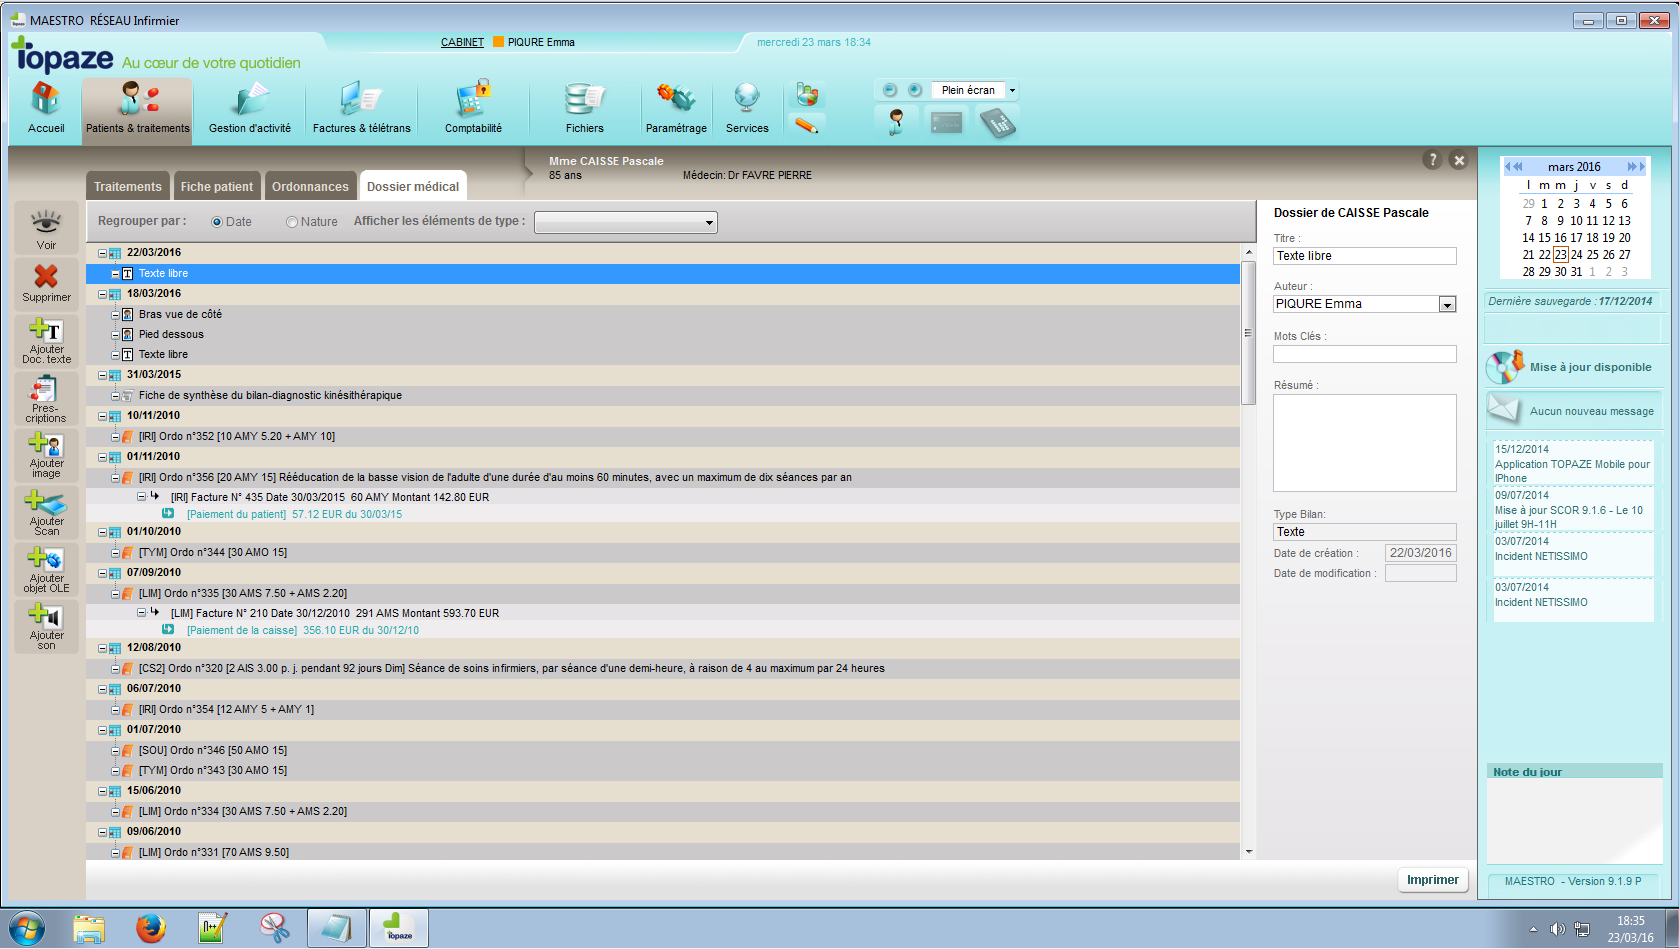
\includegraphics[width=18cm]{./img/medical_data_maestro.PNG}}
  \caption{\label{fig:dossier_medical} Dossier médical tel qu'il est présent dans Topaze Maestro.}
\end{figure}

\newpage
\begin{figure}[H]
\section*{L'éditeur de texte de Topaze Maestro}
  \centering
  \centerline{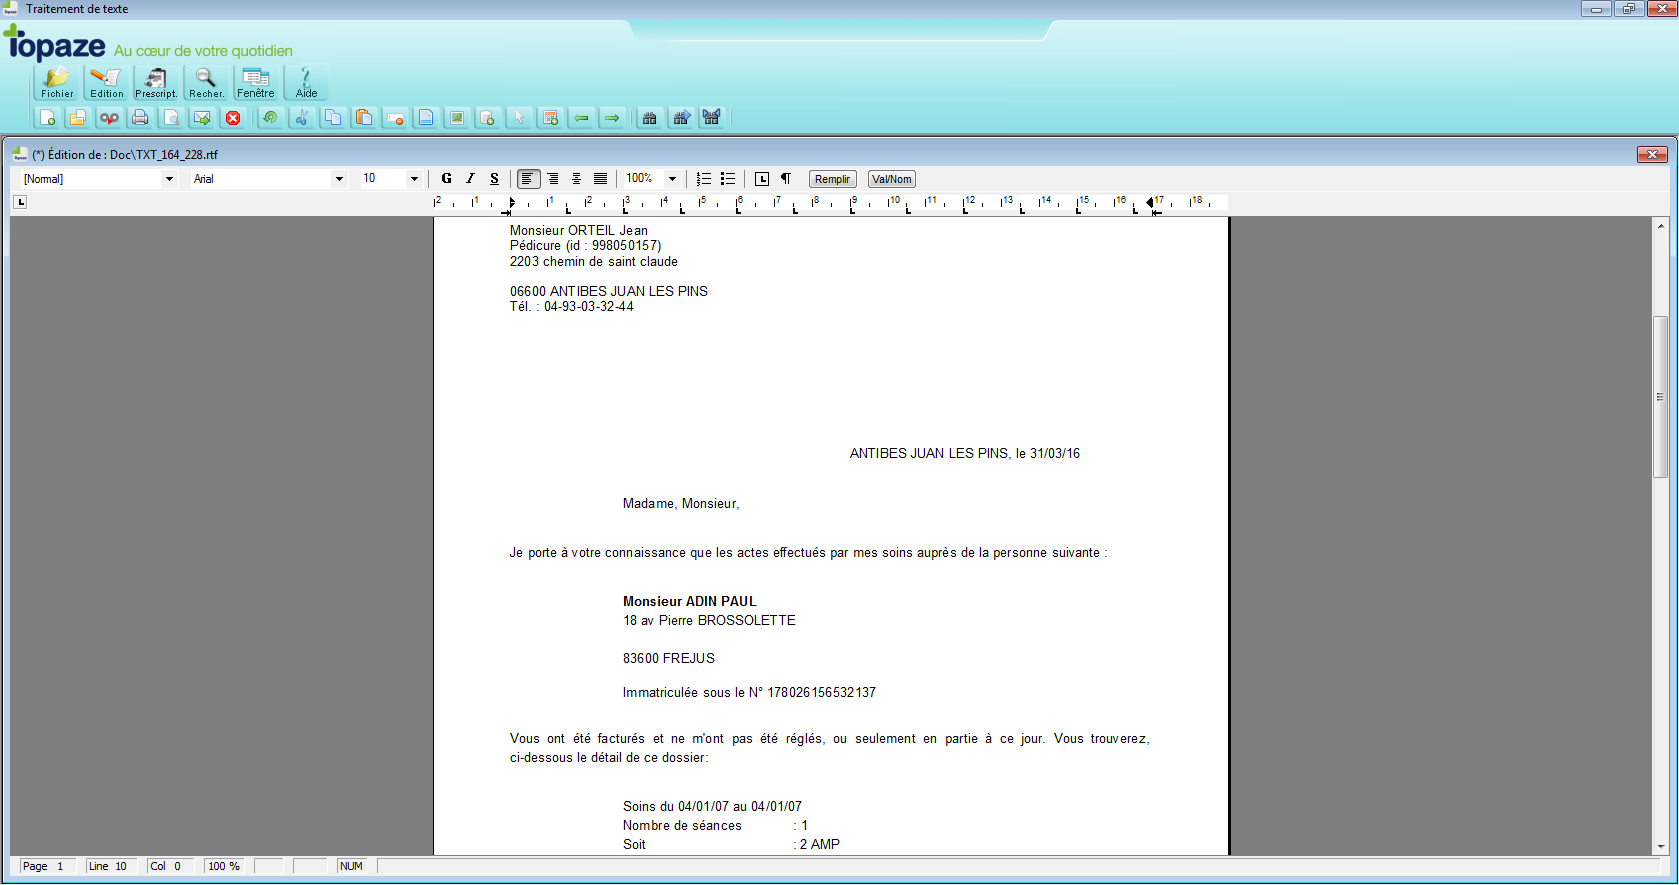
\includegraphics[width=18cm]{./img/text_editor2}}
  \caption{\label{fig:editeur_texte} L'éditeur de texte présent dans Topaze Maestro.}
\end{figure}


\newpage
\begin{figure}[H]
\section*{Exemple de modèle XML utilisé par le générateur de code}
  \centering
  \centerline{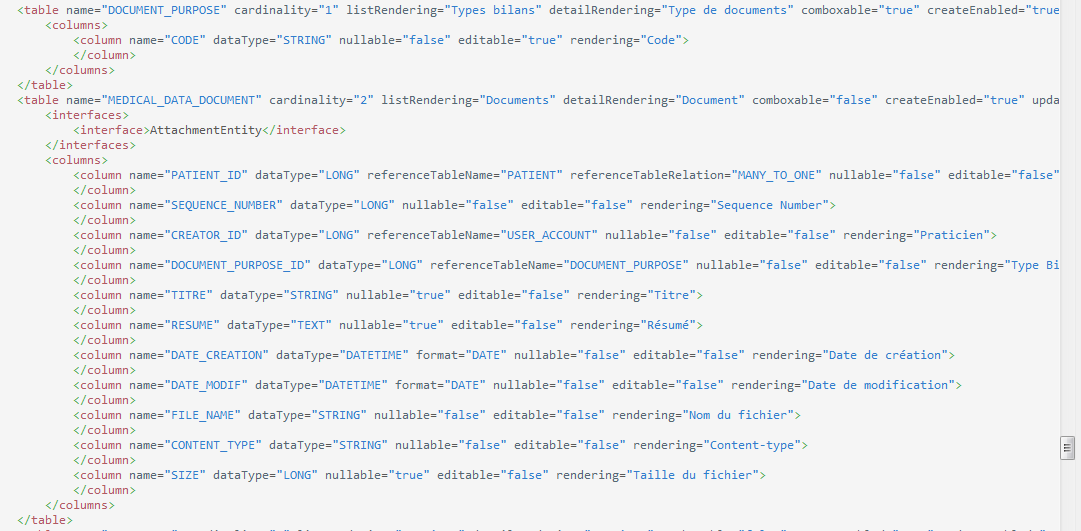
\includegraphics[width=18cm]{./img/modele_generateur}}
  \caption{\label{fig:xml} Exemple de modèle décrit en XML à destination du générateur.}
\end{figure}

\begin{figure}[H]
\section*{Diagramme de séquence de la requête d'obtention du dossier médical}
  \centering
  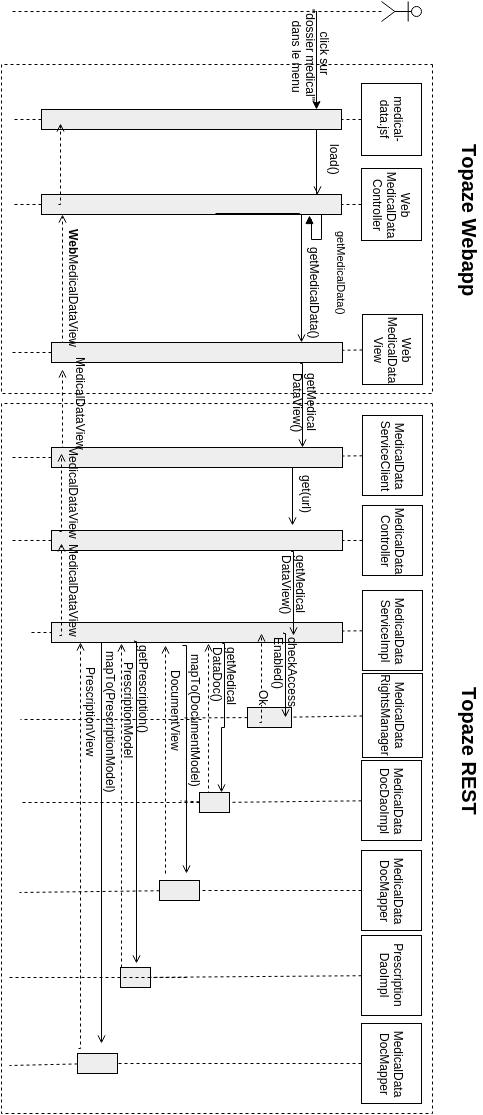
\includegraphics[height=22cm]{./img/diag_seq2}
  \caption{\label{fig:diag_seq} Diagramme de séquence modélisant la requête du dossier médical.}
\end{figure}

\newpage
\begin{figure}[H]
\section*{Le dossier médical de Topaze Web}
  \centering
  \centerline{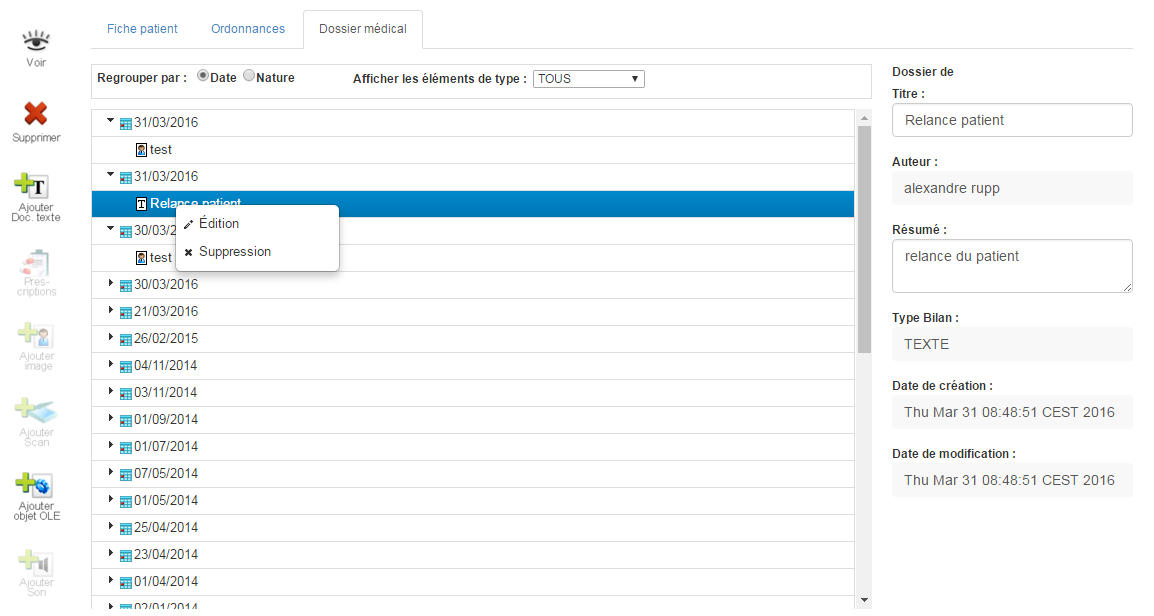
\includegraphics[width=18cm]{./img/dossier_medical_web2}}
  \caption{\label{fig:dossier_web} Le dossier médical implémenté dans Topaze Web.}
\end{figure}

\newpage
\begin{figure}[H]
\section*{L'éditeur de texte de Topaze Web}
  \centering
  \centerline{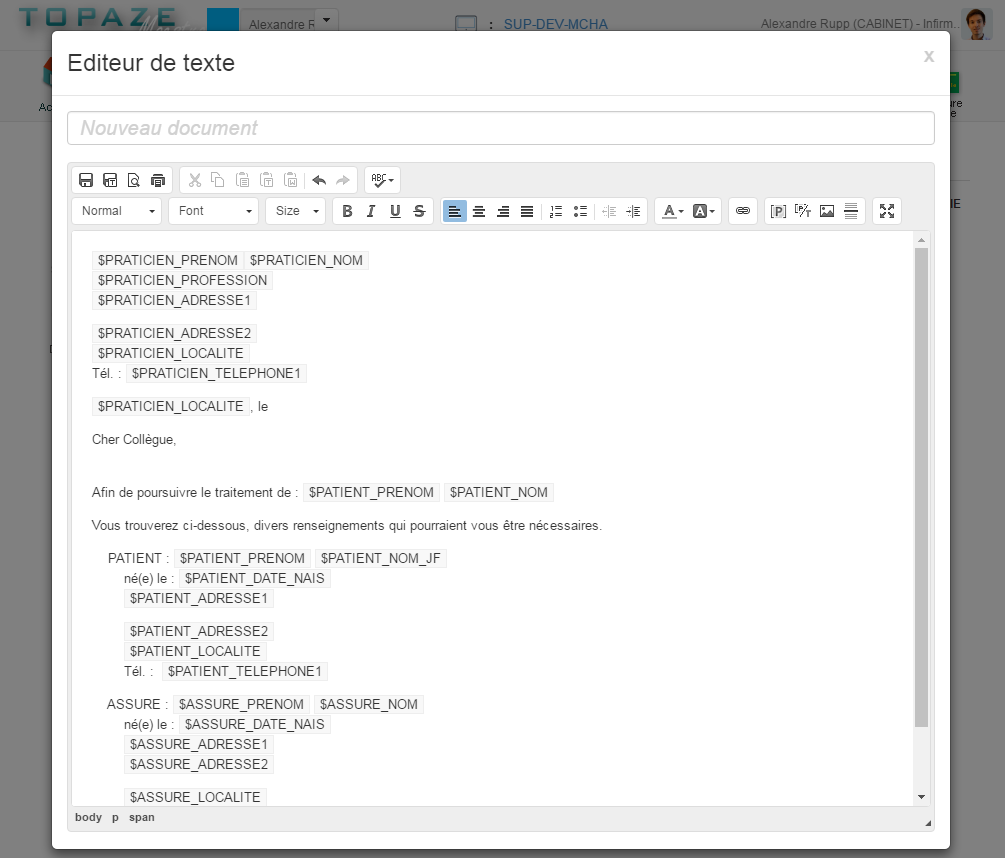
\includegraphics[width=18cm]{./img/editor2}} %editeur_topaze_web
  \caption{\label{fig:editeur_web} L'éditeur de texte (CKEditor) intégré dans Topaze Web.}
\end{figure}
%%%%%
\newpage
\begin{figure}[H]
	\section*{Prototypage de la galerie d'image}
	\centering
	\centerline{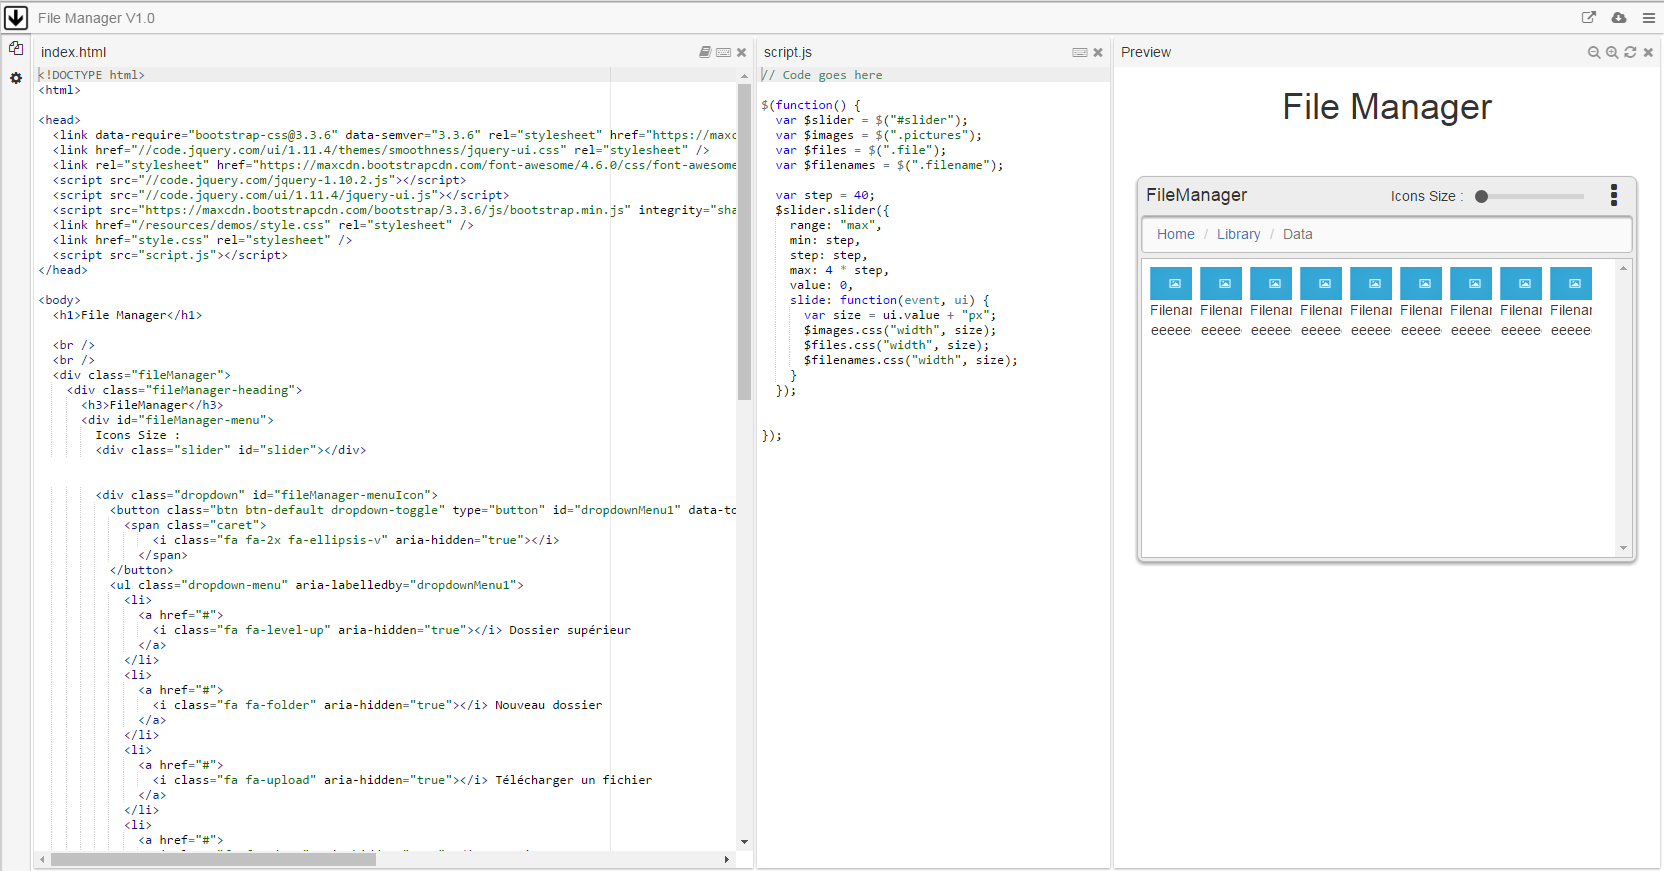
\includegraphics[width=20cm]{./img/proto_filemanager}} 
	\caption{\label{fig:proto_filemanager} Prototypage de la galerie d'image, sur plunker.}
\end{figure}

\newpage
\begin{figure}[H]
	\section*{La galerie d'image ajoutée à CKEditor}
	\centering
	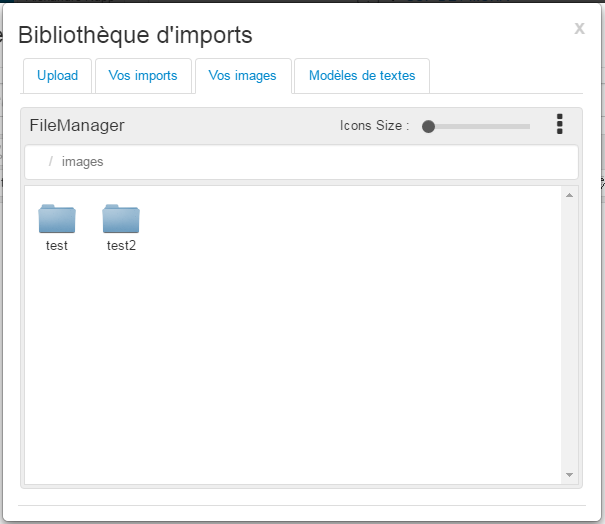
\includegraphics[width=16cm]{./img/imports} 
	\caption{\label{fig:editeur_imports} La galerie d'image ajoutée à CKEditor.}
\end{figure}


\newpage
\begin{figure}[H]
	\section*{L'arborescence des champs génériques}
	\centering
	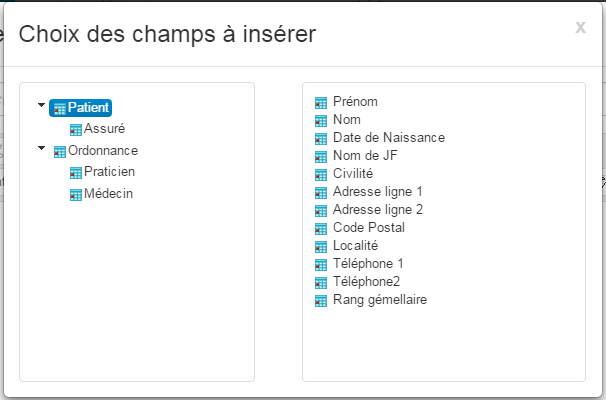
\includegraphics[width=14cm]{./img/arbo}
	\caption{\label{fig:editeur_arbo} Le plugin créé pour CKEditor pour permettre d'insérer un champ générique dans le texte.}
\end{figure}

\newpage
\begin{figure}[H]
	\section*{Le contexte associé aux champs génériques}
	\centering
	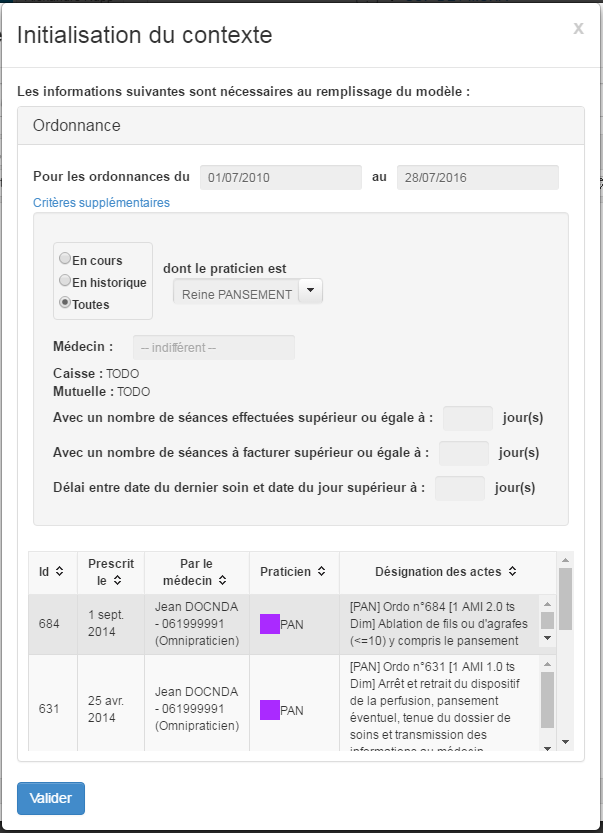
\includegraphics[width=14cm]{./img/context}
	\caption{\label{fig:editeur_context} La modale permettant de renseigner le contexte nécessaire pour remplir les champs génériques du texte. Dans le cas présent, l'utilisateur a utilisé des champs génériques de l'ordonnance. Le programme doit connaître l'ordonnance ciblée par le document.}
\end{figure}

\newpage
\begin{figure}[H]
	\section*{L'enregistrement d'un document en tant que modèle}
	\centering
	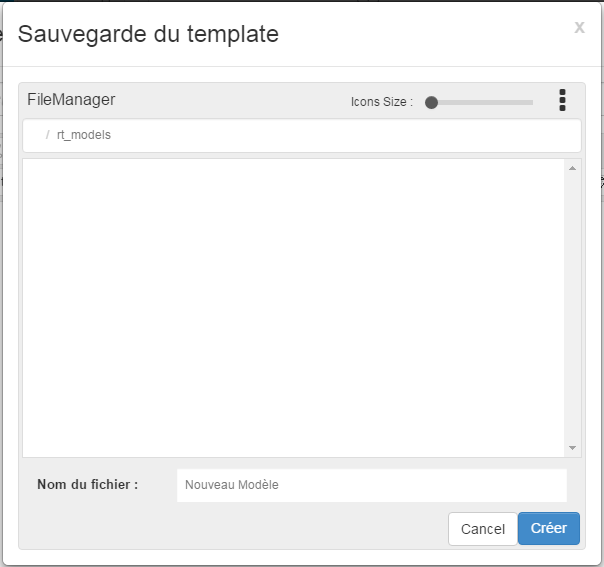
\includegraphics[width=16cm]{./img/save_template}
	\caption{\label{fig:editeur_template} La modale permettant à l'utilisateur de sauvegarder un document texte comme un modèle.}
\end{figure}

\newpage
\begin{figure}[H]
	\section*{L'écran de choix du poste utilisateur}
	\centering
	
\includegraphics[width=16cm]{./img/device}
	\caption{\label{fig:device} L'écran de choix du poste utilisateur. L'écran est affiché à la connexion (en l'absence de cookie), lors du changement de cabinet, ou lorsque l'utilisateur souhaite changer de poste utilisateur.}
\end{figure}

\newpage
\begin{figure}[H]
	\section*{L'outil de numérisation de Topaze Web}
	\centering
	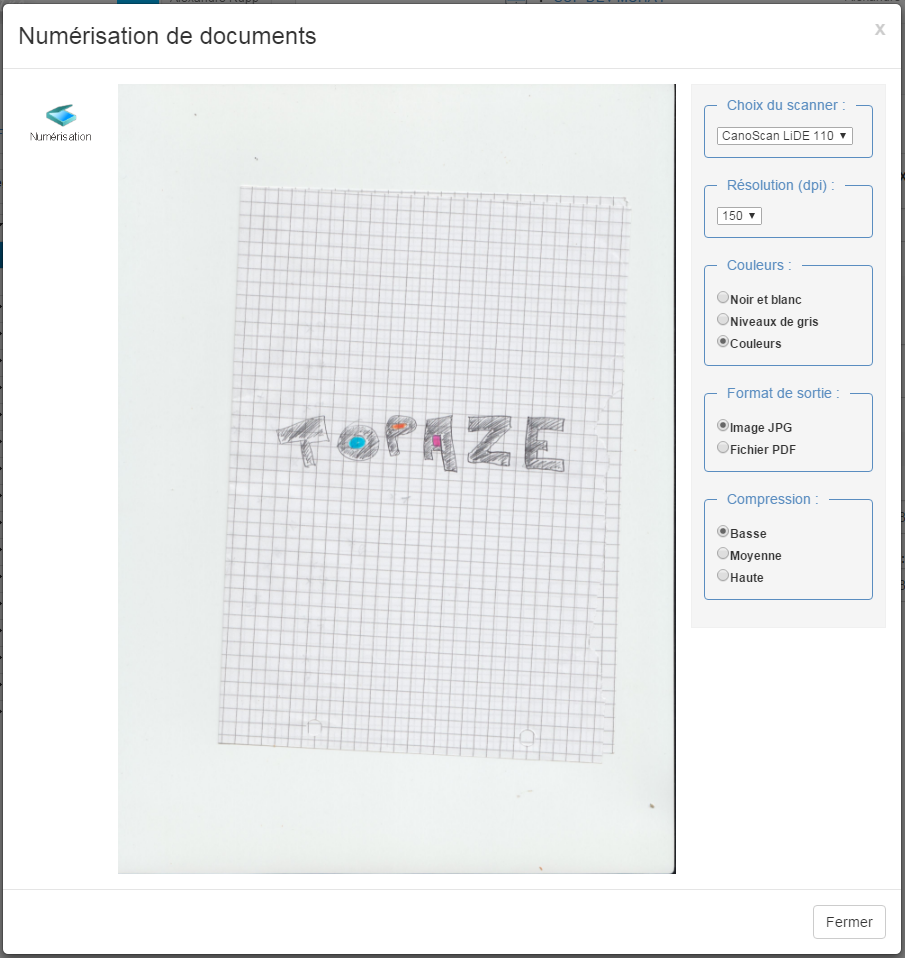
\includegraphics[width=16cm]{./img/scan}
	\caption{\label{fig:scan} L'outil de numérisation intégré dans Topaze Web.}
\end{figure}

%\newpage
%\begin{figure}[H]
%\section*{Exemple de classe annotée}
%  \centering
%  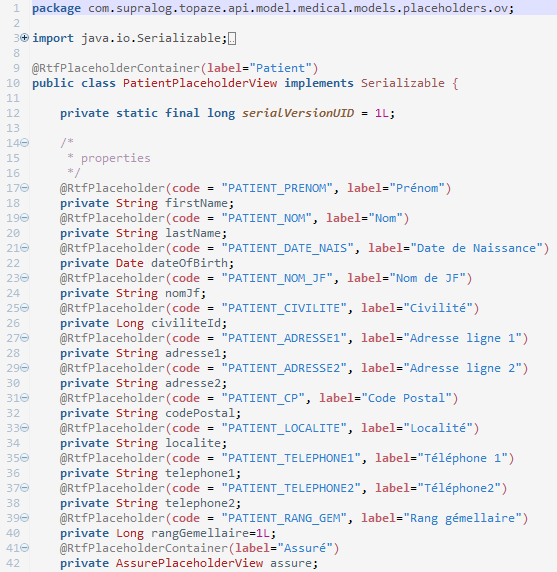
\includegraphics[width=15cm]{./img/annotations}
%  \caption{\label{fig:annotations} La classe Patient a été annotée avec 2 annotations (RtfPlaceholderContainer et RtfPlaceholder) afin de pouvoir être ensuite introspectée et servir à créer l'arborescence de placeholders.}
%\end{figure}

\end{appendices}

